\section{Introduction}
%\dan{7 pages}
\label{sec:introduction}

%\dan{this part is mostly done, only minor edits needed}

% Big data is used today in a wide range of domains, such as natural
% sciences (physics CITE, astronomy CITE, genomics CITE, biology CITE),
% social science and in particular measurements of human activity
% (e.g. recommendation CITE, personalization CITE),
% education~\cite{clauset-2015}, marketing and economics CITE, and MORE
% HERE.  The most successful type of application of Big data is {\em
%   predictive}: the data available, the \emph{seen} data, is used to
% infer a model that can predict features and trends of data that is not
% available, the \emph{unseen} data.  This potential for predictive
% analysis has generated the huge interest we see today in Big data, and
% has, in some sense, democratized data, by stimulating a huge number of
% ``data enthusiasts'' to collect, explore, analyze, integrate, and
% visualize data.  The term Big data is often used today to refer not
% just to the traditional features like volume, variety, velocity, but
% also to its wide availability to a broad range of users.


% lg1 - original commentout below at end; take care as this can lead to confusion

Much of the success of Big data today comes from
  \emph{predictive or descriptive analytics}: statistical models or data mining algorithms applied to data
  to predict new or future observations, e.g., we observe how users click on ads, then build a model and predict how future
  users will click.
Predictive analysis/modeling is central to many scientific fields, such as bioinformatics and natural language processing,
  in other  fields - such as social economics, psychology, education and environmental science - researchers are focused
  on testing and evaluating {\em causal hypotheses}.
While the distinction between causal and predictive analysis has been recognized, the conflation between the two is common.

\ignore{
Both predictive and causal analysis are needed to generate and test theories,
  policy and decision making and to evaluate hypotheses, yet each plays a different role in doing so.
In fact, performing predictive analysis to address questions that are causal in nature could lead to a flood of false discovery claims.
In many cases, researchers who want to discover causality from data analysis settle for predictive analysis either because they think it is causal or lack of available alternatives.
}
Causal inference has been studied extensively in statistics and
computer science \cite{Fisher1935design,Rubin2005,holland1986statistics,PearlBook2000\ignore{,Spirtes:book01}}.
Many tools perform causal inference
 using statistical software such as R project. However, in this demonstration we show that, these toolkits do not scale to large datasets.  Furthermore, in many of the most interesting Big Data settings, the data
is highly relational (e.g, social networks, biological networks, sensor networks and more) and likely to pour into SQL systems. There is a rich ecosystem of tools and organizational requirements that encourage this. Transferring
data from DBMS to statistical softwares or connecting these
softwares to DBMS can be error prone, difficult, time consuming and inefficient. For these
cases, it would be helpful to push statistical methods for causal inference into the DBMS.
\ignore{\corey{should go over the scalability / current tool problem here before jumping into the solution?}}

In this demonstration we propose \GSQL,\footnote{ The prefix Zali refers to
  al-Ghzali (1058-1111), a medieval Persian philosopher. It is known
  that David Hume (1711-1776), a Scottish philosopher, who gave the
  first explicit definition of causation in terms of counterfactuals,
  was heavily influenced by al-Ghzali's conception of causality
  \cite{shalizi2013advanced}.}
  a SQL-based framework for drawing causal inference that circumvents the scalability issue with the existing tools. ZaliQL supports state-of-the-art methods for causal
inference and runs at scale within a database engine.   \GSQL\ is designed and implemented as an extender for PostgreSQL object-relational database
system and includes a series of optimization techniques allowing our system to
scale to billions of records. In this demonstration we use \GSQL\ to perform causal inference in the following scenario:

\ignore{
\begin{table*}[!htb] \scriptsize
    \begin{subtable}{.5\linewidth}
      \centering

       \begin{tabular}[t]{|l|l|}
  \hline
  % after \\: \hline or \cline{col1-col2} \cline{col3-col4} ...
  \bf{Attribute}   & \bf{Description}  \\  \hline
  FlightDate & Flight date   \\ \hline
  UniqueCarrier	& Unique carrier code   \\ \hline
  OriginAirportID & 	Origin airport ID  \\ \hline
  CRSDepTime & Scheduled departure time  \\ \hline
  DepTime & Actual departure time \\ \hline
    & difference in minutes between   \\
  DepDelayMinutes & scheduled and actual departure \\
   & time. Early departures set to 0  \\ \hline
  LateAircraftDelay & Late aircraft delay, in minutes  \\ \hline
  SecurityDelay & Ssecurity delay, in minutes \\ \hline
  CarrierDelay & Carrier delay, in minutes  \\ \hline
  Cancelled & Binary indicator  \\
  \hline
\end{tabular}
     \caption{Flight dataset}
    \end{subtable}%
    \begin{subtable}{.5\linewidth}
      \centering


       \begin{tabular}[t]{|l|l|}
  \hline
  % after \\: \hline or \cline{col1-col2} \cline{col3-col4} ...
  \bf{Attribute}   & \bf{Description}  \\  \hline
  Code  & Airport ID    \\ \hline
  Date	& Date of a repost   \\ \hline
  Time        & Time of a report  \\ \hline
  Visim        & Visibility in km  \\ \hline
  Tempm & Temperature in C$^{\circ}$ \\ \hline
  Wspdm         & Wind speed kph \\ \hline
  \ignore{Precipm         & Humidity \% \\ \hline}
  Pressurem         & Pressure in mBar  \\ \hline
  Precipm         & Precipitation in mm  \\ \hline
  \ignore{Rain & Binary indictor    \\ \hline
  Snow & Binary indictor \\ \hline}
  Tornado & Binary indictor \\ \hline
  Thunder & Binary indictor \\ \hline
  Hum & Humidity \% \\ \hline
  Dewpoint & De point in  C$^{\circ}$ \\ \hline
\end{tabular}
        \caption{Weather dataset}
    \end{subtable}
 \vspace{-0.1cm}   \caption{\bf{List of attributes from the flight(a) and weather(b)  datasets that are relevant to our analysis.}}
\label{tab:attlist}
\end{table*}
}
\begin{figure}
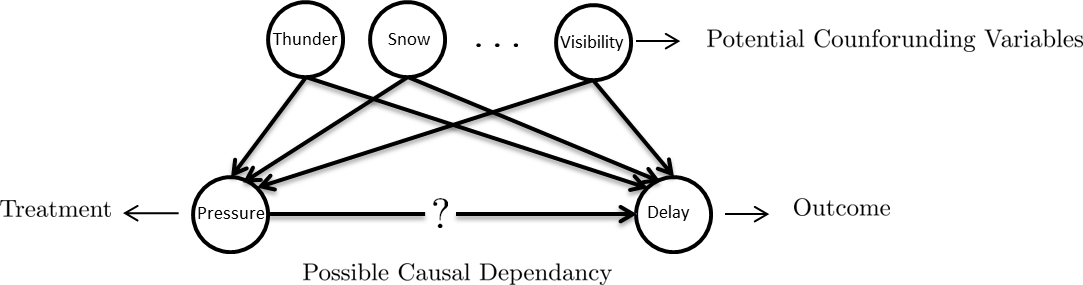
\includegraphics[scale=0.5]{figures/counf.png}
\caption{A typical scenario for causal hypothesis testing}

\label{fig:cv}
\vspace{-0.3cm}
\end{figure}
\begin{figure}
  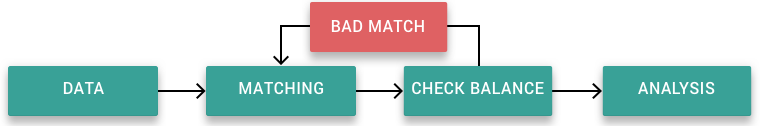
\includegraphics[scale=0.3]{Figures/Matching-Flowchart.png}
\caption{Matching observational data for Causal inference}
\label{fig:flowchart}
\vspace{-0.3cm}
\end{figure}


\begin{example} \em \delay \ \em
Flight delays pose a serious and widespread problem in the United States and
 significantly strain on the national air travel system, costing society many billions of dollars each year \cite{ball2010total}.
The upsetting impact of weather conditions on aviation is well known, however quantifying
  the causal impact of different weather types on flight delays at different airports is essential for evaluating
  approaches to reduce these delays.
Even though predictive analysis, in this context, might help make certain policies, this problem is causal.
We conduct this causal analysis as a running example through this demonstration.
To this end, we acquired flight departure details for all commercial flights within the US from 2000 to 2015
  (105M entries) and integrated it with the relevant historical weather data (35M entries).
These are relatively large data sets for causal inference that can not be handseled by the existing tools.
\end{example}
\ignore{
Table \ref{tab:attlist} presents the list of attributes from each data set that is relevant to our analysis.
}

\ignore{
We argue that this problem is causal in nature and performing
a predictive analysis can be very misleading. To conduct the analysis, we collect the flight and weather data
since 2005.
The flight data is acquired from the US Department of
Transportation [117] and consists of 168 million rows. The
weather data is gathered using the weather underground API 2
and consists of 10 million rows
Suppose we are interested in the impact of
low pressure on flight departure delay at X airport.
To highlight the distinction between predictive and causal nalsysis
Suppose we are interested to see if weather low pressure
has any impact on departure delay at X airport. By conducting a
}

\ignore{
This analysis is causal in nature. For example,
when we concern about the effect of low pressure on flight
departure delay, we are not interested in the difference
between average flights departure delay when low
barometric pressure is reported at the flight
time and the average flight departure delay when high
pressure is reported. Rather, researchers are interested
to find out weather low/high barometric pressure has any causal
impact on flight departure delay and if so, to compute the strength of that effect.
To say it in a somewhat different way, the observed distribution of
the flight departure delay, for instance,  at John F. Kennedy International Airport (JFK) in 2015 is an outcome of a complicated stochastic process. When we make
a probabilistic prediction of the departure delay, $Y$,  by
conditioning on low/high barometric pressure,\ignore{\footnote{ Barometric pressure above 1022.69 and below  1009.14 millibar is usually considered as high and low pressure respectively \cite{barometricpressureheadache:article}.}} $X$ (low barometric pressure (=1) vs. hight barometric pressure (=0))- whether we predict $\E[Y | X = x]$ or
$Pr(Y | X = x)$, with $x \in \{0,1\}$, or something more
complicated- we are just filtering the output of
the mechanisms that controlled the flight departure
delay at JFK in 2015, picking out the cases where they
happen to have set $X$ to the value $x$, and looking
at what goes along with that. In fact, by applying this
naive predictive analysis, we obtain that
$E(Y | X = 1)-E(Y | X = 0)\backsimeq 4$, which suggests that
barometric pressure affected the flight departure delay at
JFK in 2015 and might be a good predictor for that.}

When we make predictive analysis, whether we predict $\E[Y | X = x]$ or $\textrm{Pr}(Y | X = x)$ or
  something more complicated, we want to know the conditional distribution of $Y$ given $X$.
On the other hand, when we make a causal analysis, we want to understand the distribution of $Y$, if the
  usual mechanisms controlling $X$ were intervened and set to $x$.
In other words, in causal analysis we are interested in {\em  interventional} conditional distribution,
  e.g., the distribution obtained by (hypothetically) enforcing $X = x$ uniformly over the population.
In causal analysis, the difficulty arises from the fact that here the objective is to estimate (unobserved)
  {\em counterfactuals} from the (observed) {\em factual} premises.

%interface screenshots
\begin{figure*}[t]
  \begin{subfigure}{0.33\linewidth}
    \centering
    \hspace{-.6cm}
    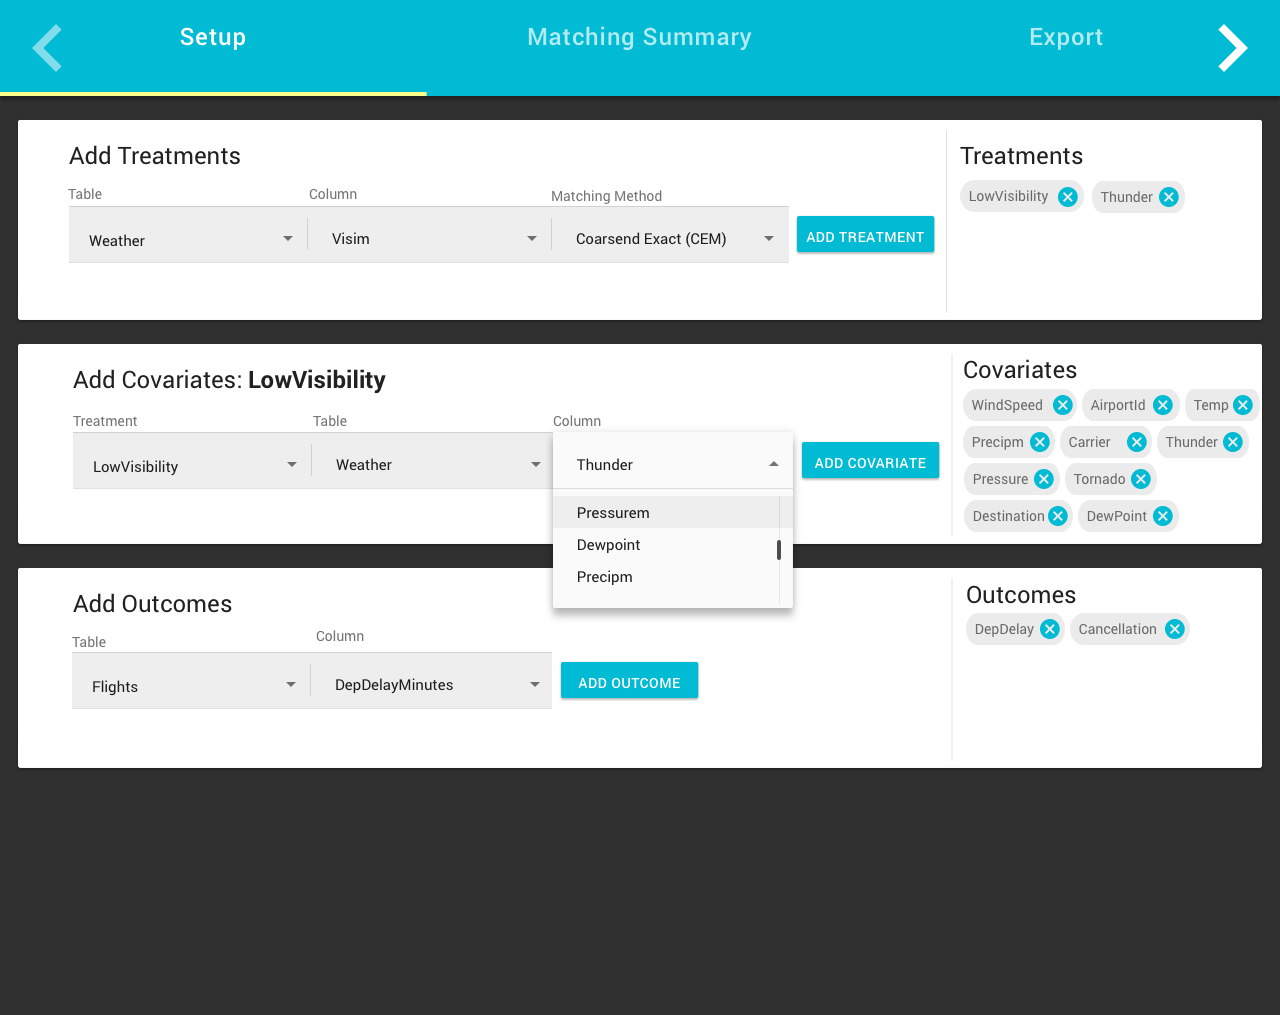
\includegraphics[scale=0.13]{Figures/Setup.png}
    \caption{\scriptsize }
    \label{sfig:testaa}
  \end{subfigure}\hfill
  \begin{subfigure}{0.33\linewidth}
    \centering
    \hspace{-.6cm}
    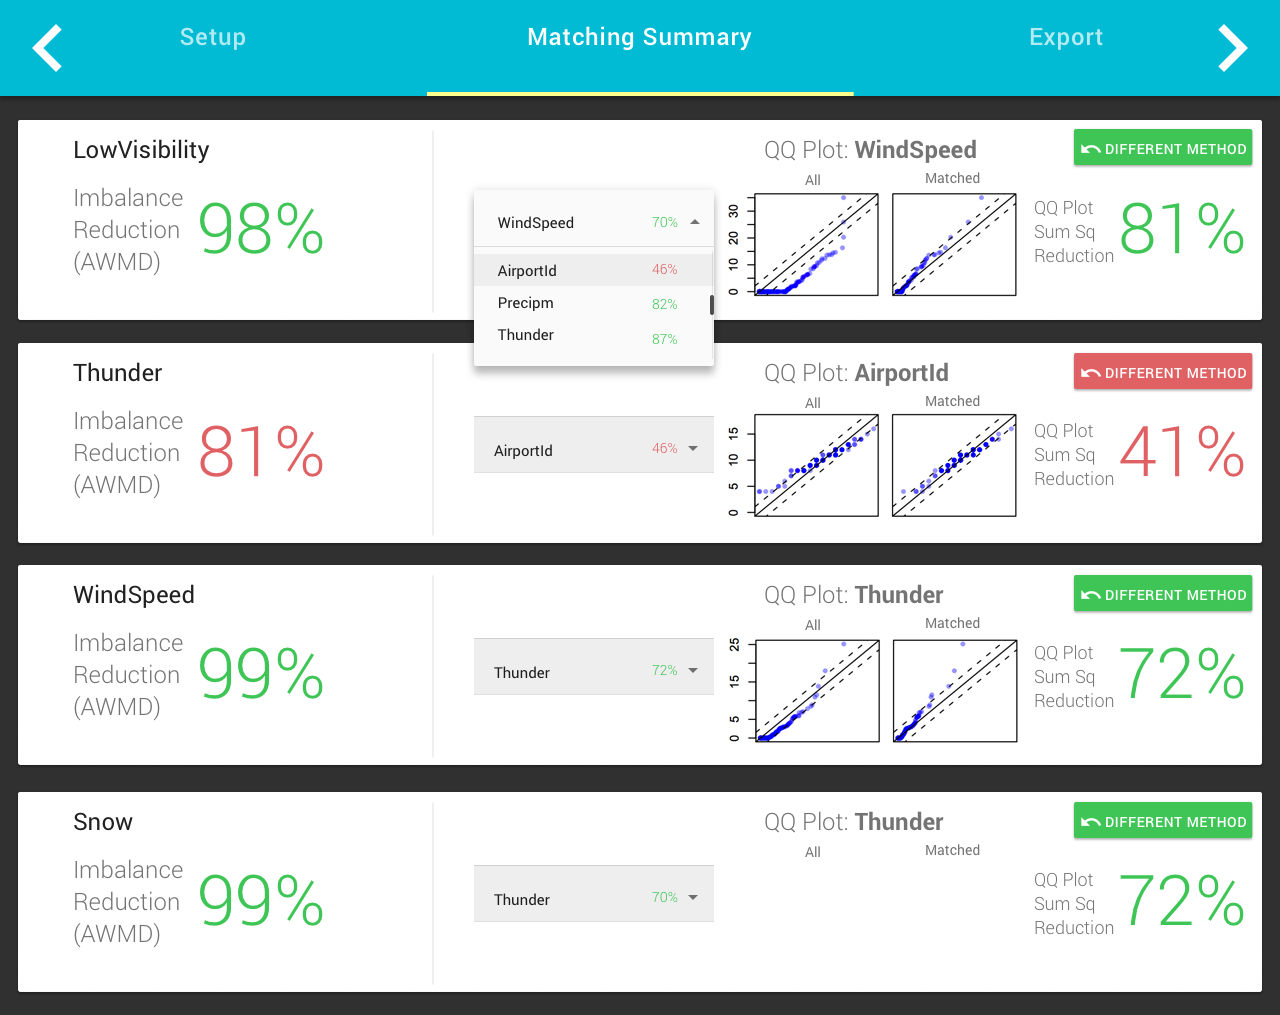
\includegraphics[scale=0.13]{Figures/Matching-Summary.png}
    \caption{\scriptsize }
    \label{sfig:testbb}
  \end{subfigure}\hfill
  \begin{subfigure}{0.33\linewidth}
    \centering
    \hspace{-.6cm}
    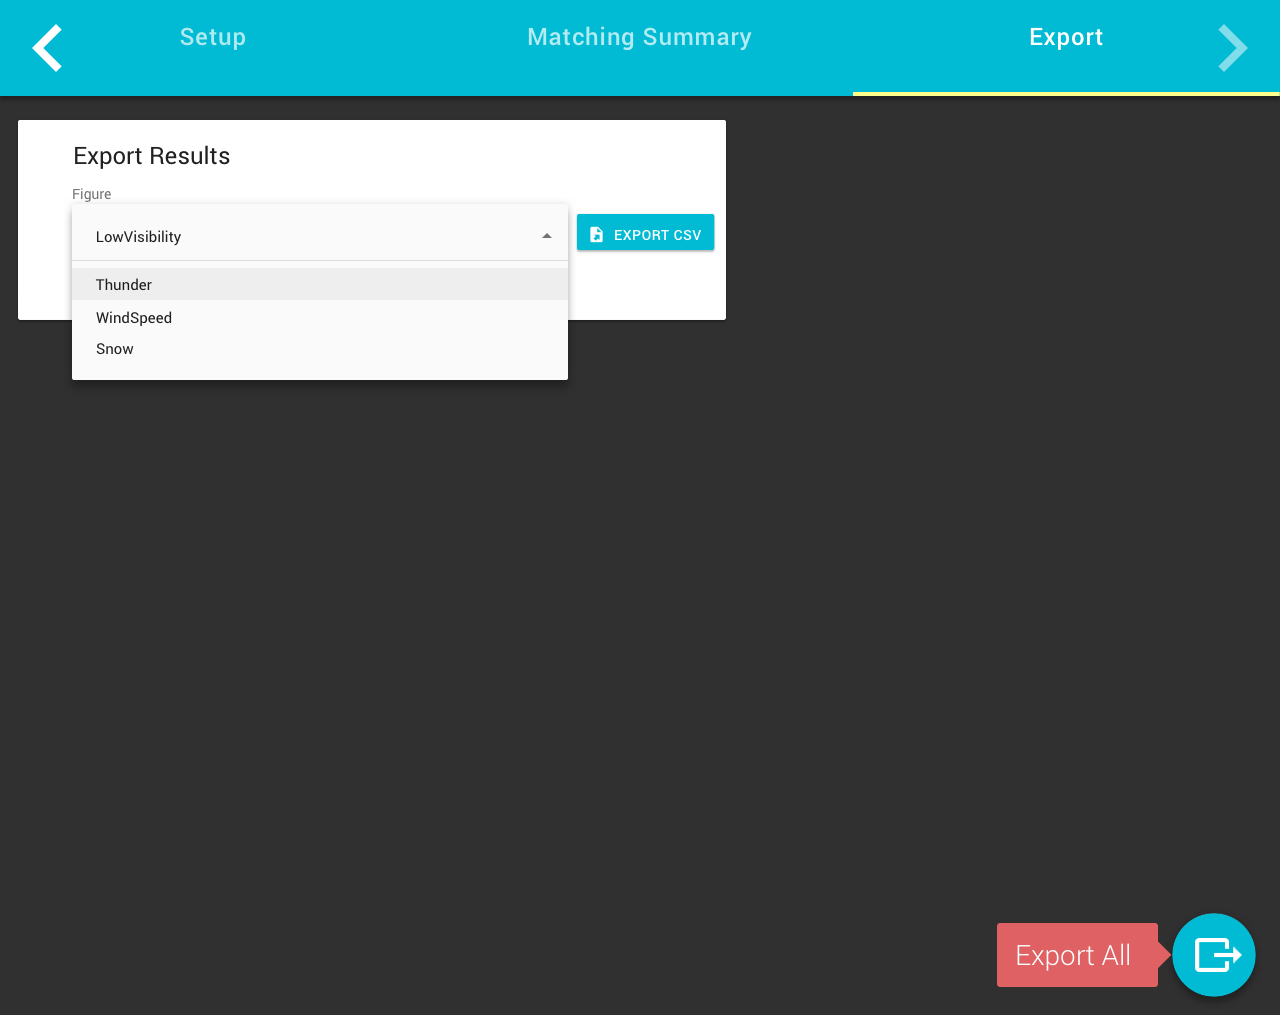
\includegraphics[scale=0.13]{Figures/Export.png}
    \caption{\scriptsize }
    \label{sfig:testcc}
  \end{subfigure}\hfill
\caption{Demonstration screenshot described in Section \ref{sec:dd} \babak{We have plenty of space to use bigger fonts. it is barley retable}}
\label{fig:inteface}
\vspace{-0.3cm}
\end{figure*}


It is known that causal inference is possible under careful random \emph{randomized} or \emph{controlled} experiment, in which a treatment (the potential cause) is assigned randomly to subjects. However, most of the big data available today are observational, meaning that unlike collected opportunistically. The major problem in causal inference from observational data is the existence of the so-called {\em confounding variables} which makes the direct comparison between the group that received treatment and the group that are subject to control impossible. The following example explains this issue.



\begin{example} \em \delay (cont.) \ \em   Suppose we want to explore the effect of the low-pressure (treatment) on flight departure delays (outcome).  The direct comparison of
flight delay between the those flight that happen during low-pressure (treated groups) and the opposite group is misleading.  It is known that high pressure is generally associated with clear weather,    while low-pressure is associated with unsettled weather, e.g.,
    cloudy, rainy, or snowy weather\ignore{\cite{weba2,barometricpressureheadache:article}}. Thus, as shown in Figure \ref{fig:cv}, factors such as thunder, snow, visibility confound pressure and delay. Therefore, conducting any sort of predictive analysis identifies
    low-pressure as a predictor for flight delays. 
  However, low-pressure does not have any causal impact on departure delay
    (low-pressure only requires longer takeoff distance) \cite{FAA08}. In this demonstration, by conducting a careful causal analysis using \GSQL\, we show that low-pressure is only a correlated attribute with flight delays and has no significant causal impact on flight delay.
    
    \ignore{By performing a careful casual analysis
    \GSQL\ found that other attributes such as thunder, low-visibility, high-wind-speed and
    snow have the largest causal effect on flight delays (see Sec. \ref{sec:endtoend});
  this is confirmed by the results reported by the FAA.}
\end{example}


% They defined a very simple model, where we
% want to conclude \dan{Lise: what's your comment here?}  if one
% variable, called ``treatment'' causes one particular output variable,
% called ``effect'', and have developed a rich set of techniques for
% that purpose.  The end goal of their analysis is to establish the
% average causal-treatment effect.  More recently, in the AI literature
% Pearl~\cite{pearl2010introduction,PearlBook2000} has extended this
% simple model by introducing {\em causal networks}, and developing a
% logical framework for reasoning about causality.  Their aim is to
% enable complex inference in a network of causal associations.  While
% the ultimate goal is the same, to check whether a particular input
% causes a particular outcome, the methods deployed are different from
% those in statistics.

\vspace{-0.1cm}

\ignore{
This paper makes the following specific contributions: we describe a
suite of techniques for expressing the existing advanced methods for
causal inference from observational data in SQL that run at scale
within a database engine (Section \ref{sec:BasicTechniques}). Note
that we do not claim any contribution the existing methods; we
introduce several optimization techniques that significantly speedup
causal inference, both in the online and offline setting (Section
\ref{sec:OptimizationTechniques}); we validate our system
experimentally, using real data from the U.S. DOT and Weather
Underground \cite{flightdata,Weatherdata}
}


Roughly speaking, in order to draw a valid causal conclusion one need to control for the
confounding influences that affect both treatment and outcome. Papular methods for 
performing this task in statistic and social science are {\em subclassification and matching} \cite{Rubin1983b,IacKinPor09,rosenbaum1984reducing}.
The key goal of matching is to prune  data so that
the remaining data have better balance between the treated and control groups meaning that the empirical distributions of the confounding variables (a.k.a, covariates) in the groups are more similar.  Since there is no generic metric to compare
two distributions, measures such as mean, skewness, quantile and multivariate histogram are used for this purpose. A rule of thumb is to evaluate different distance metrics and
matching methods until a well-balance matched subset with
a reasonable size obtained \cite{IacKinPor09}. Figure \ref{fig:flowchart} summarized the tasks involved with causal inference from observational data.


This demonstration will enable the attendees to experiment with various methods for causal inference and experience their benefits and limitations.
The attendees will select a causal question by specifying a treatment,
  an outcome and particular method to perform causal inference.
The attendee will also able to adjust the tunable parameters for these algorithms. The demonstration will run a remotely served web application that interfaces with our demo flight and weather database.

The demonstration will make two contributions. It will
  (1) explain why machine leaning methods fail to distinguish causation and correlation 
  (1) explain and demonstrate the pipeline of drawing valid causal conclusions from data and
  (2) enable the attendees to experience different methods for causal inference and investigate their proc and cons.
